\section{Project management}
\subsection{Science research project management}
Scientific research projects cannot be project-managed in the way that many other technical activities can. Research is, by its nature, unpredictable.  In research, one does not know exactly what will be found, where it will be found, or how long it will take to find. So, MSL manages research in a flexible way that provides transparency and allows projects to evolve and adapt. 

MSL maintains a portfolio of science projects that are reviewed annually to ensure research goals and strategies remain sensible and robust. The review process is intended to raise the visibility of these activities within MSL and to encourage discussion and engagement across the laboratory. The reviews also provide an opportunity to consider future resourcing requirements. 

Every year, projects give a brief presentation (Tea-Time-Talk), summarising activities in the recent past (12-18 months) and outlining proposed activities (12-18 months). The audience is MSL. A written summary is prepared. The presentation documents (slides and summary) are retained from year to year, to capture project outcomes and evolution. 

New R\&D proposals present an explanation of the project and how it sits within MSL’s strategies. Again, a written summary, together with presentation slides, is retained. Sizeable projects may need to provide a “road map” of anticipated milestones and resourcing requirements over a longer time span, so that an initial assessment of programme feasibility can be made.

In evaluating projects, it is as impossible to pick “winners” as is it is to identify “losers”. Nevertheless, there are some basic attributes of a good project:
\begin{itemize}
\item Natural Inclination:  A project that harnesses the natural inclinations, interests and expertise of the individuals involved will yield considerably better results than a directed approach. 

\item Benefit to MSL: Research activities and goals will align with MSL’s strategy and contribute to the development of informal-knowledge and expertise. 

\item Feasibility: Projects will be financially and logistically feasible. The resources required must be reasonable, including capital equipment, laboratory space, FTE, etc.

\item Quality and Diversity: It is unwise for MSL to concentrate research activities and resources narrowly; but it is also unwise to support research activities of poor quality. Projects should (or, in the early stages, have the potential to) deliver high-quality research outcomes (~see figure~\ref{f:science_review}~).
\end{itemize}


\begin{figure}[ht]
\centering
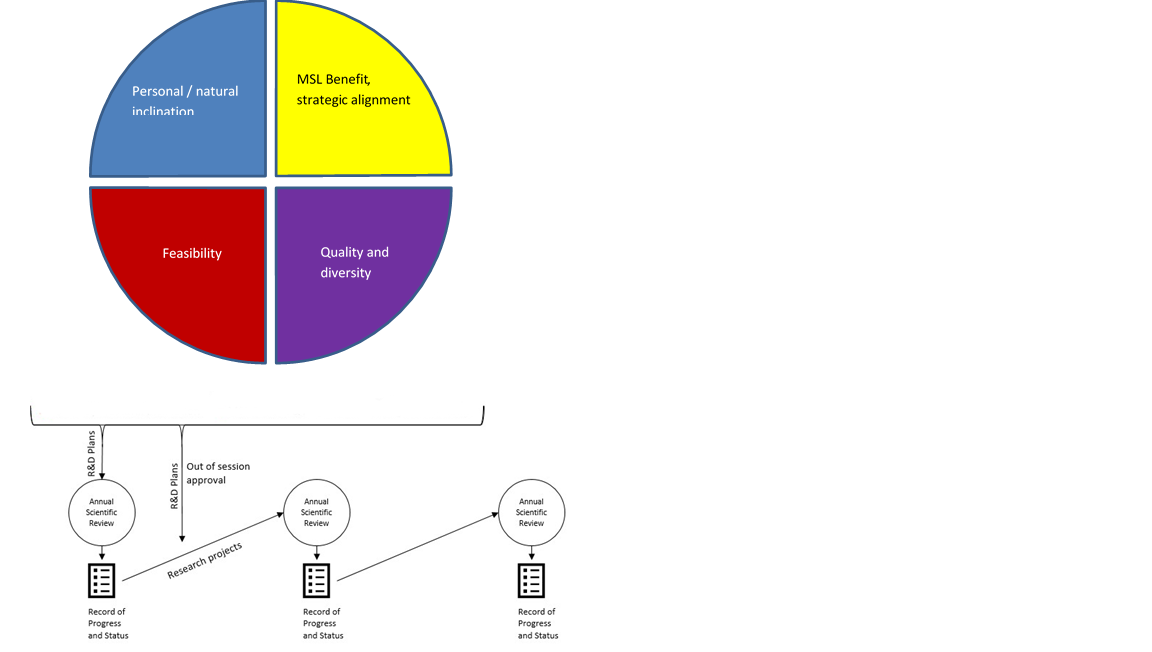
\includegraphics[scale=1]{pictures/science_review}
\caption{A schematic representation of science research project policy.}
\label{f:science_review}
\end{figure}
